\chapter[Referencial Teórico]{REFERENCIAL TEÓRICO}

\section{Gamificação}

Gamificação é um termo relativamente novo e foi utilizado pela primeira vez em 2002 por \cite{pelling} e usado a primeira vez em documentações no ano de 2008 e vem ganhando repercussão há alguns anos \cite{deterding2011gamification}.

Diversos autores definem o termo, as definições em sua maioria são similares, algumas são colocadas a seguir: Gamificação é o ato de aplicar os prícipios e mecanismos de design de jogo em ambientes de não jogo \cite{kumar2013gamification}.
\cite{da2014gamificaccao} define gamificação como a ação de se pensar como em um jogo, utilizando as sistemáticas e mecânicas do ato de jogar em um contexto fora de jogo. Para \cite{deterding2011gamification} gamification é o uso de design de jogos em contextos de não jogo. 

A Figura (\ref{deterdingfig}) ilustra o pensamento de Deterding, que diferencia jogos sérios de gamificação e jogos de brincadeiras e interações lúdicas. A composição de jogos utilizada por ele é similar a proposta por \cite{mcgonigal2011reality}, formada por metas, regras, sistema de feedback e participação voluntária. Jogos sérios não são feitos para entrenimento, mas assim como a gamificação, são feitos para contextos de não jogo. A figura ilustra a separação e ao mesmo tempo a similaridade entre dos itens discutidos. 


\begin{figure}[h]
	\centering
		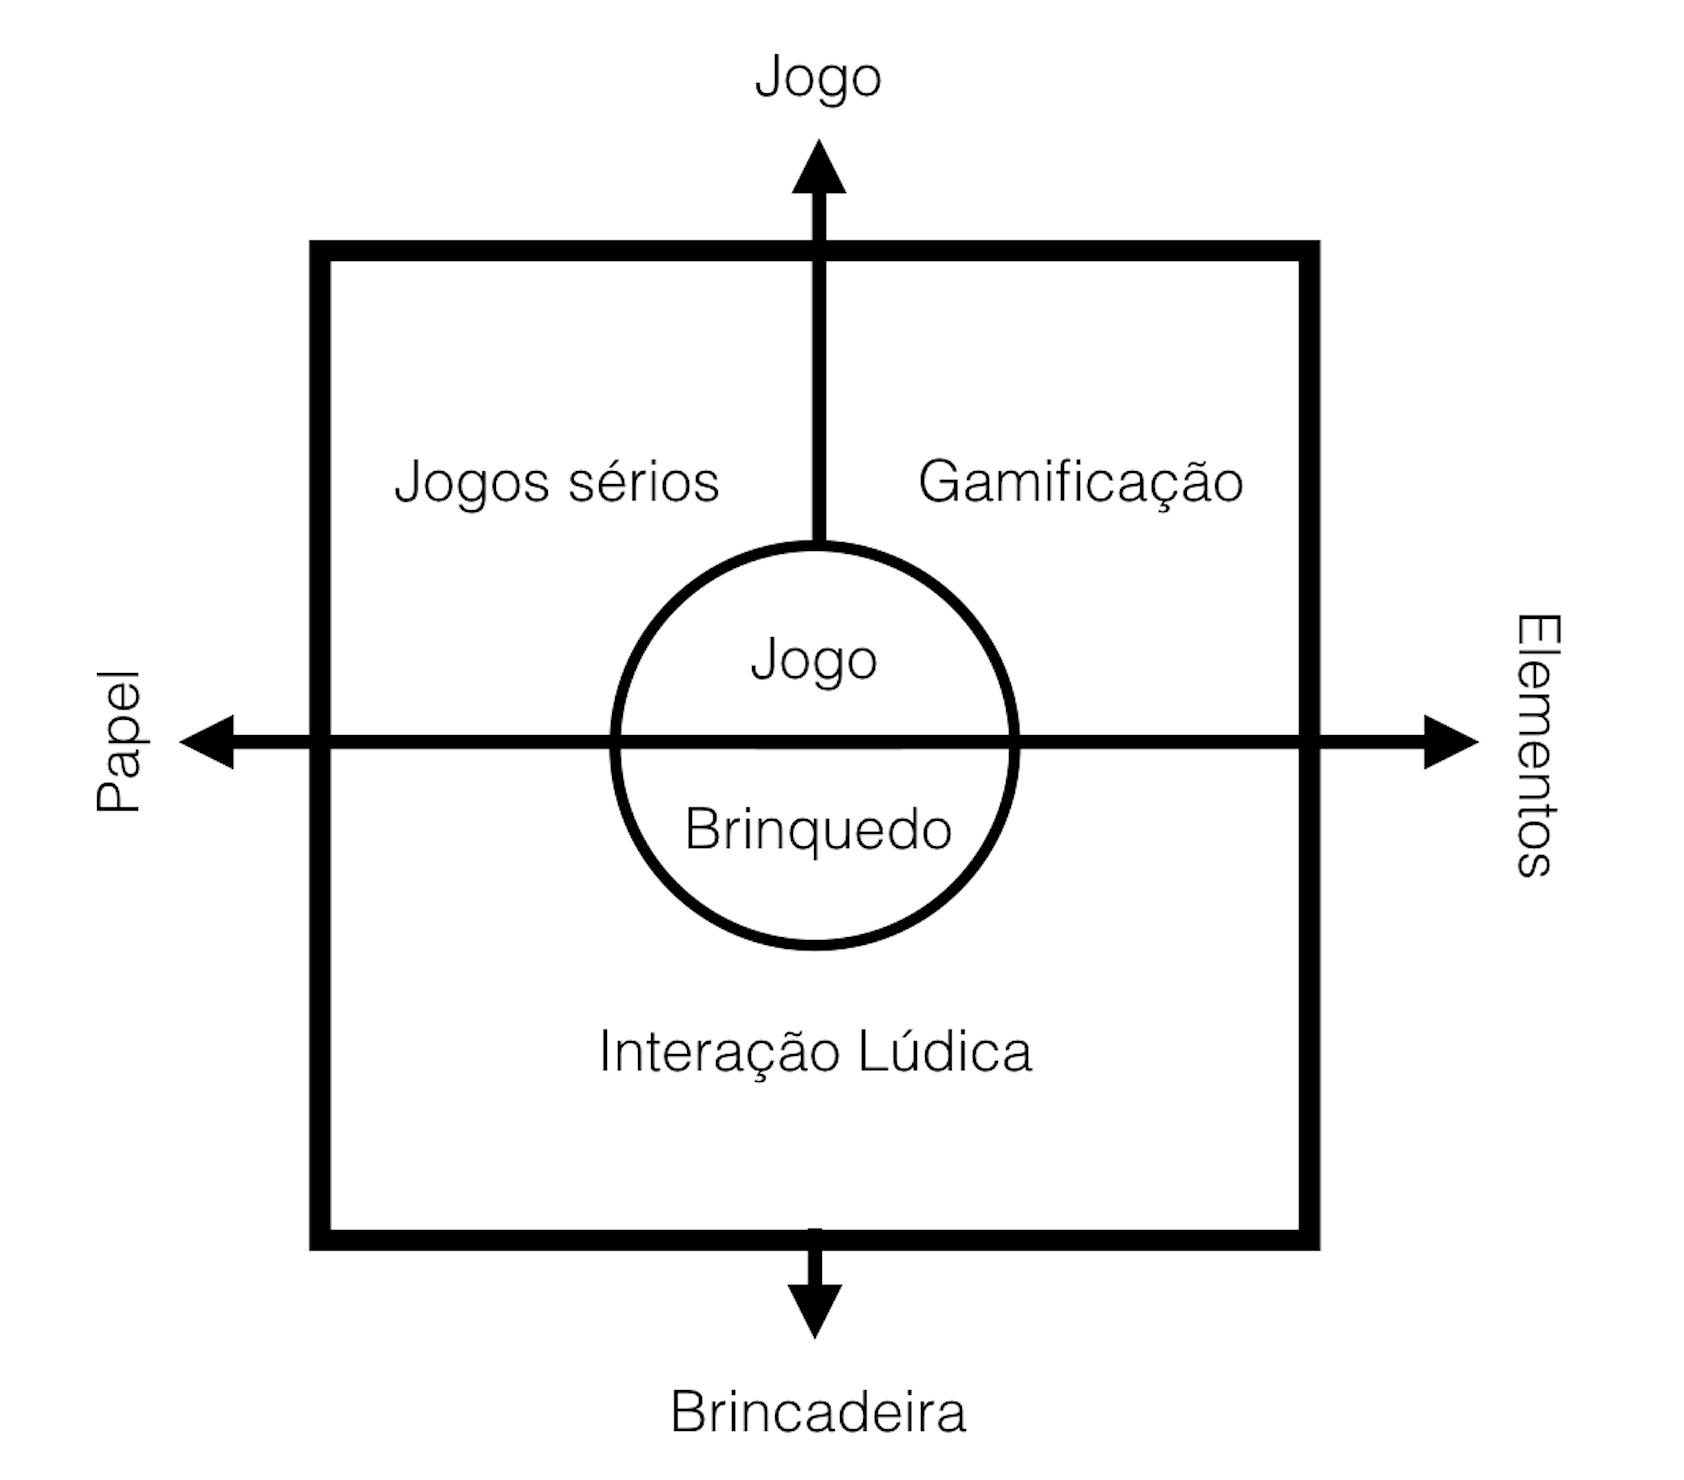
\includegraphics[keepaspectratio=true,scale=0.3]{figuras/deterding.png}
	\caption{Definição detalhada de gamificação. Fonte: \cite{deterding2011gamification}.\label{deterdingfig}
}
\end{figure}

\newpage


 Em contraponto, \cite{chou2015actionable} diz que o termo gamification é muito abrangente e discutir a semântica da palavra não é produtivo.  Segundo \cite{zichermann2011gamification}, gamificação pode ter significado diferente, para diferentes pessoas. Chou e Zichermann afirmam que gamificar é mais que inserir elementos no seu site, ou inserir troféus, pontos e medalhas em um contexto, é preciso uma abordagem mais ponderada e motivadora. Incorporar elementos e mecânicas de jogos não fazem o jogo ser divertido, a simples aplicação destes elementos pode deixar o jogo tedioso e acarretar em um fracasso.

 O termo gamificação é novo, mas o ato de construir algo parecido com um jogo não \cite{chou2015actionable}, os estudo dos aspectos interessantes nos jogos também não, na década de 80 já se estudava porque jogos de computadores são tão cativantes e como deixar outras interfaces tão cativantes quanto \cite{malone1982heuristics}, na época três estudos foram realizados afim de se responder tais questões, a conclusão foi que os aspectos cativantes eram desafio, fantasia e curiosidade. 

As mecânicas dos jogos não são o verdadeiro motivo de um jogo ser engajado. A motivação do usuário vem antes, é necessário pensar no que se deseja que o usuário sinta \cite{chou2015actionable}. Apesar de não achar produtiva a discussão sobre o que é gamificação Chou também a define, porém de maneira um pouco diferente, para ele gamificação é o ato de derivar a diversão e o engajamento tipicamente encontrados em jogos. Essa será a definição utilizada para a construção desde trabalho.


\section{Frameworks de Gamificação}

\subsection{Modelo de Bartle}

Para \cite{bartle1996hearts} existem quatro perfis de jogadores, as pessoas costumam se inclinar ao menos um pouco para cada um dos perfis, mas acabam tendo preferência por um. Essa conclusão foi feita após um estudo relacionado a jogos multiusuário. Para ele as pessoas dentro desse contexto apreciam realização dentro do jogo, a exploração, a socialização com outras pessoas e a imposição sobre os outros. Os quatro perfis de jogadores identificados pelo autor são:



\begin{itemize}
\item  \textbf {Conquistadores}: O aumento de nível e a soma total de pontos é o principal objetivo deste jogador dentro do jogo. Exploração é necessário apenas para acumular pontos. Socialização é um método de descobrir como ganhar pontos. Matar outros jogadores ou personagens só se faz necessário se isso servir para acumular mais mais pontos. Para o empreendedor o importante é acumular.
\item  \textbf {Exploradores:}  Gostam de descobrir o jogo, seguir caminhos não tradicionais, descobrir como as coisas funcionam. Marcar pontos pode ser necessário para se descobrir uma nova fase, mas pode ser tedioso e qualquer um com metade de um cérebro pode fazê-lo, matar pode ser divertido, mas pode ficar chato se alguém vem cobrar vingança, socializar pode servir para descobrir coisas novas, mas geralmente não é isso que ocorre. Para o explorador a verdadeira diversão vem da descoberta.
\item  \textbf {Socializadores: } Estão interessados nas outras pessoas do jogo e no que elas tem a dizer. O jogo é apenas um plano de fundo, um terreno comum onde as coisas acontecem para os jogadores. Explorar pode ser necessário a fim de entender o que todo mundo está falando. Acumular ou adquirir pontos pode ser exigido para ter acesso a outros níveis . Matar, só se for estritamente necessário. O objetivo para os socializadores é conhecer pessoas e construir relacionamentos.
\item  \textbf{Assassinos:} Os com perfil de assassinos querem se impor sobre os outros, mas não é o perfil mais recompensador. Quando maior a massa de sofrimento, maior a satisfação. Adquirir pontos pode ser necessário para ficar mais poderoso, a exploração é necessária para descobrir novos jeitos de matar e a socialização pode ser necessária para descobrir novas táticas. O objetivo é causar emoções ruins nos outros jogadores.
\end{itemize}

\begin{figure}[h]
	\centering
		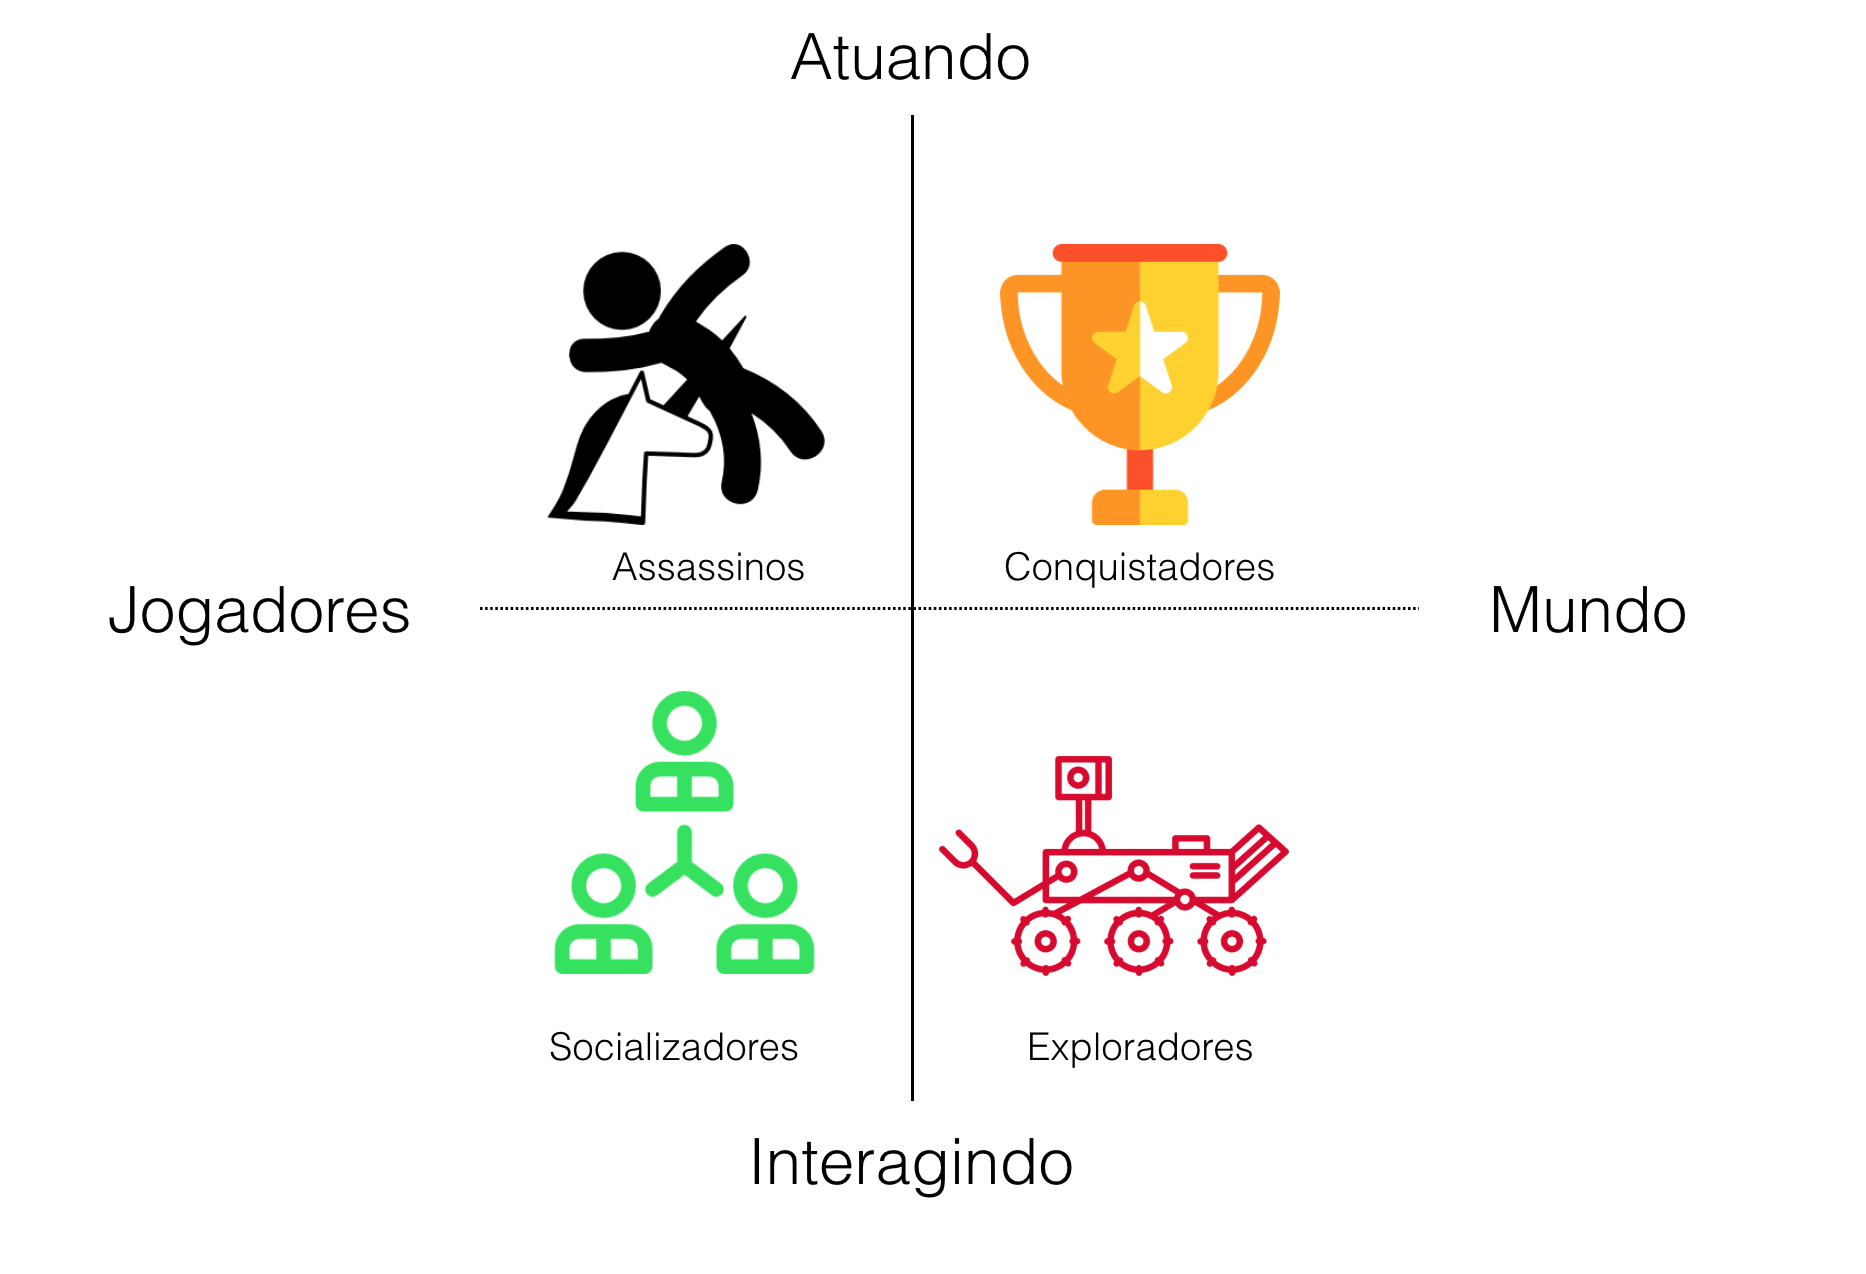
\includegraphics[keepaspectratio=true,scale=0.35]{figuras/bartlefig.png}
	\caption{Perfis de jogadores. Adptado: \cite{bartle1996hearts}.\label{bartlefig}
}
\end{figure}

 Os eixos do gráfico representados na Fig.(\ref{bartlefig}) representam os interesses dos jogadores. O eixo x enfatiza no quadrante da esquerda e o ambiente no quadrante da direita. Os extremos do gráfico são as quatro preferências. 

 Os conquistadores estão interessados em atuar sobre o mundo, dominar o jogo. Os exploradores estão interessados em interagir com o mundo e nas surpresas que o jogo pode ter. Os socializadores estão interessados em interagir com outros jogadores. Os assassinos estão interessados em atuar com outros jogadores, nem sempre com o consentimento do outro. O gráfico de interesse é uma representação do que os jogadores estão interessados em um jogo multijogador.
 

\subsection{Modelos centrados no ser humano}

Design centrado no ser humano ou design centrado no jogador trata de por o usuário e seus objetivos no centro do processo e desenvolvimento da gamificação, o que gera produtos alinhados as necessidades do usuário \cite{kumar2013gamification}. Design focado no ser humando é um termo melhor para gamificação, otimizar a motivação humana no sistema é o oposto de otimizar puramente a eficiência, pessoas não são engrenagens rudimentares \cite{chou2015actionable}.

\subsubsection{Modelo de Kumar}

A figura (\ref{pcdfig}) representa o modelo de gamificação sugerida por Kumar. Primeiro é preciso entender o lugar no qual o jogador está inserido, o sucesso da gamificação depende disso, por isso design centrado no ser humano. Após o entendimento do contexto se dá o entendimento da missão que envolve o entendimento do contexto do cenário de negócio, identificando, por exemplo, o negócio desejado e assim construir uma missão apropriada. O modelo proposto pode ser abstraído, mas é focado em negócios. Enquanto se define a missão é necessário estudar o jogador e suas motivações, as informações descobertas podem impactar a gamificação.

 Após todo o entendimento feito é necessário aplicar as mecânicas de jogos. As mecênicas de jogos são os aspectos mais visíveis da gamificação e precisam ser selecionadas baeadas na motivação do jogador. A missão precisa ser gerenciada, a motivação monitorada e as mecânicas mensuradas continuamente \cite{kumar2013gamification}.

\begin{figure}[h]
	\centering
		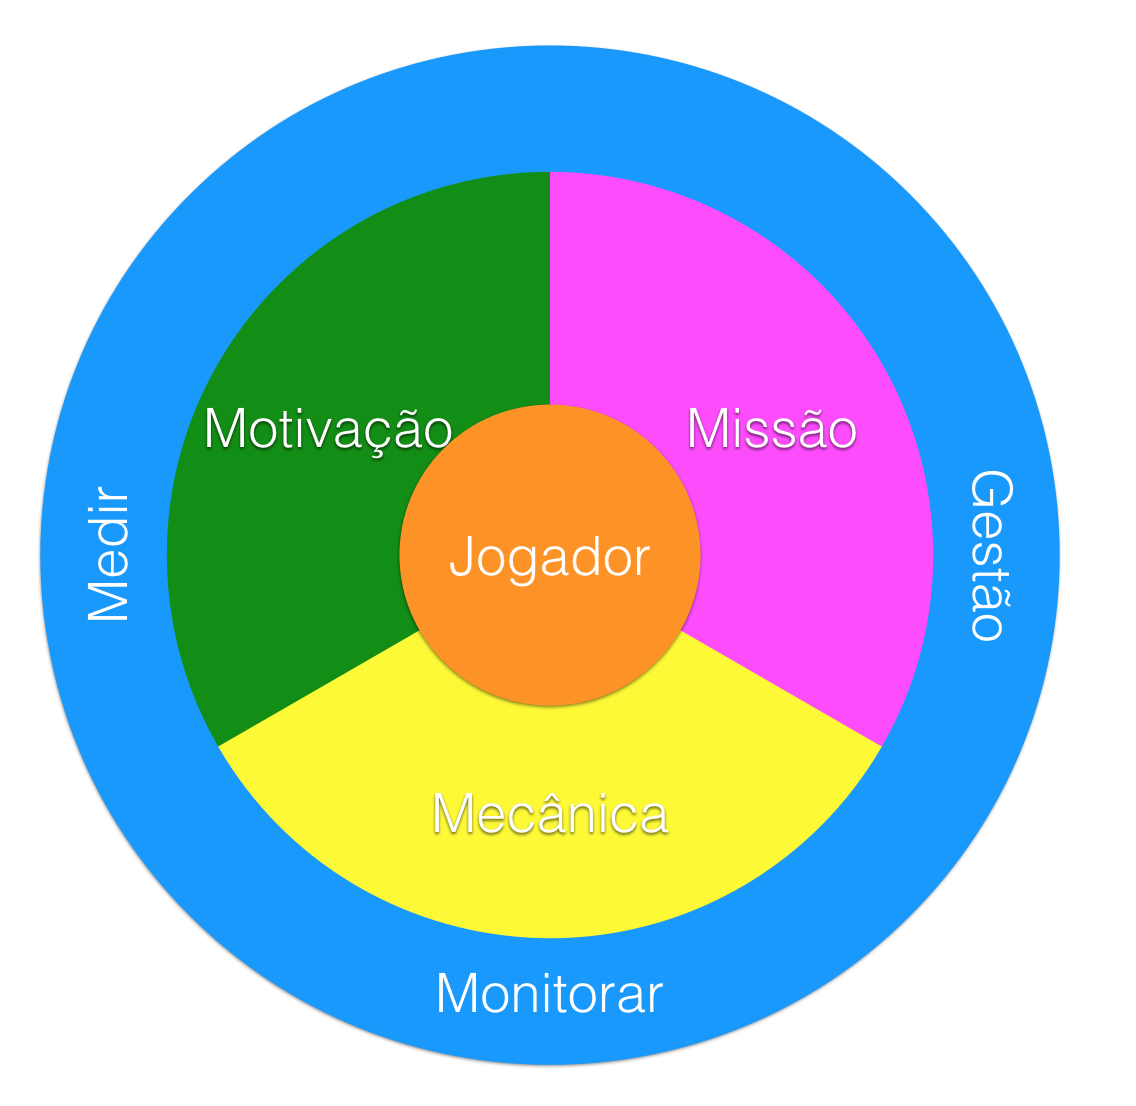
\includegraphics[keepaspectratio=true,scale=0.35]{figuras/pcd.png}
	\caption{Design centrado no ser humano. Adptado: \cite{kumar2013gamification}.\label{pcdfig}
}
\end{figure}

\subsubsection{Modelo de Yu-kai Chou}

Para \cite{chou2015actionable}, a motivação do usuário vem antes de tudo, a proposta de design focado no ser humano vai contra o pensamento de foco no funcional, que deseja obter resultador rápidos, para o autor, a industria de jogos foi a primeira a adotar esse pensamento. Os jogos não tem outra proposta senão o ser entreter o ser humano.

Chou é um dos percussores na área de gamificação, muito do que o autor transmite foi fruto de experiência pessoal, segundo ele, os jogos mudaram a sua vida e desde então ele estuda para poder explicar como fazer jogos mais significativos e como tornar a vida mais divertida e a resposta encontrada é gamificação. 

Para tornar a gamificação acessível o autor criou o octalysis framework, que recebeu este nome por ser um octagono composto de oito unidades principais (UP). As UPs representam as motivações principais e segundo Chou, se não há nenhuma das UPs por tráz de uma ação não há motivação e nada acontecerá. As unidades principais são compostas de técnicas de gamificação, \cite{chou2015actionable} define técnicas de gamificação como When I mention Game Techniques, I mean techniques that incorporate Game Elements (which includes Game Mechanics) to drive motivation.

 O framework é representado na Fig(\ref{octfig})

\begin{figure}[h]
	\centering
		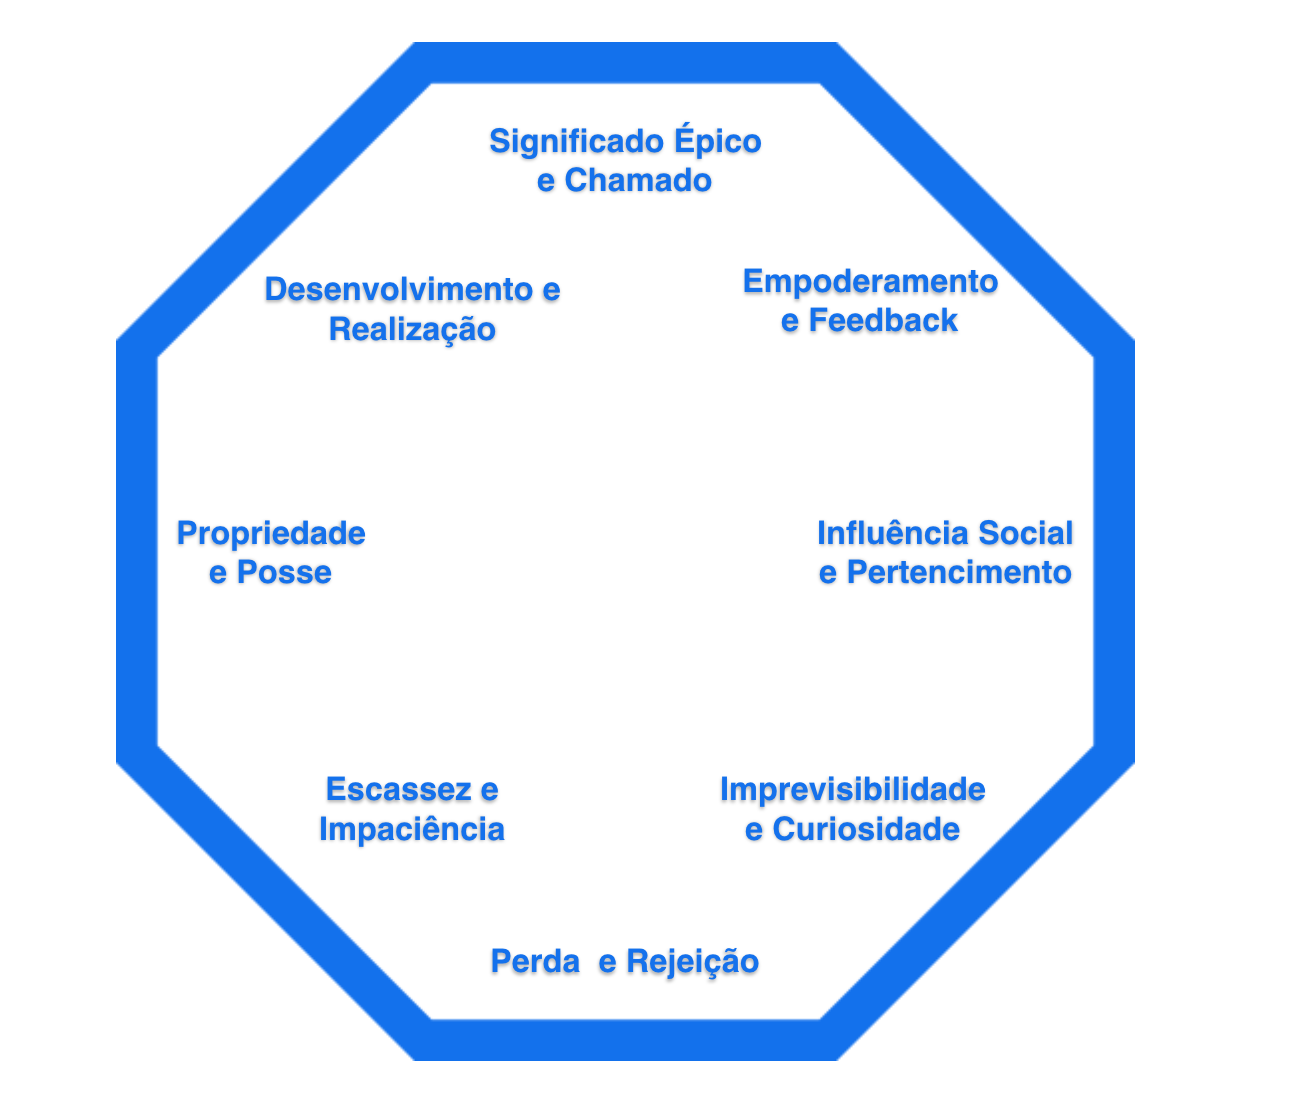
\includegraphics[keepaspectratio=true,scale=0.5]{figuras/octfig.png}
	\caption{Octalysis Framework. Fonte:  \cite{chou2015actionable}.\label{octfig}
}
\end{figure}

\newpage

A primeira unidade principal é denominada significado épico e chamado, uma definição para esta UP pode ser representada por uma analogia, por exemplo, quando uma pessoa acredita que está fazendo algo maior que si própria ela está sendo motivada por esta UP. Esta unidade principal não é sobre fazer o usuário se sentir feliz, é sobre um significado maior, para se ter uma visão mais elevada. 

Um exemplo de aplicação desta UP pode ser visto nos contribuintes de software livre e nas pessoas que constroem a wikipédia. A unidade significado épico e chamado faz as pessoas se sentirem engajadas em algo maior que elas, elas sentem que contribuir faz a diferença. Algumas técnicas dessa unidade principal são exemplificadas abaixo:

\begin{itemize}
\item  \textbf{Narrativa}: Oferece ao jogador algum contexto sobre o porque ele deveria jogar o jogo;
\item  \textbf{Sorte de Iniciante:} Faz o jogador acreditar que ele é bom no jogo assim que ele se inicia e possui uma capacidade que os outros jogadores não possuem;
\item  \textbf{Herói da Humanidade:} Faz o jogador acreditar que ele pode ajudar os menos privilegiados, dentro do contexto.
\end{itemize}

A segunda unidade principal é desenvolvimento e realização, esta UP recebe a maioria dos itens relacionados a gamificação, como medalhas, barras de progresso, pontos. É uma UP que diz respeito ao desenvolvimento de habilidades, por exemplo, quando um professor oferece uma estrela por a um aluno por uma atividade realizada corretamente, ela está motivando o aluno fazendo o mesmo se sentir realizado. Algumas técnicas dessa unidade principal são exemplificadas abaixo:

\begin{itemize}
\item  \textbf{Barras de Progresso:} Informam o progresso de alguma unidade de medida do contexto do jogo;
\item  \textbf{Efeito Estrela de Rock:} Faz o usuário se sentir como se fosse uma estrela do rock;
\item  \textbf{Oásis no Deserto:} Faz o usuário acreditar que depois daquela oportunidade o jogo acaba.
\end{itemize}

A terceira unidade principal é empoderamento da criatividade e feedback, ela é o porque das brincadeiras com lego e fazer arte serem atividades divertidas, é a UP da criatividade e motiva as pessoas a utilizá-la, como quando eram crianças e montavam e desmontavam legos repetidamente. Algumas técnicas dessa unidade principal são exemplificadas abaixo:

\begin{itemize}
\item  \textbf{Mecânica Sempre Verde:} Fornece a continuidade do jogo de maneira natural, sem que necessariamente coisas novas sejam acrescentadas;
\item  \textbf{Escolha de Percepção:} Escolher a partir de diferentes opções, as pessoas preferem escolher que ter apenas uma opção;
\item  \textbf{Escolhas Significativas:} Opções que representam algo significativo e demonstram preferências que não são obviamente superiores as outras.
\end{itemize}

A quarta unidade principal é propriedade e posse, motiva o usuário fazendo com que ele se sinta dono ou no controle de algo e faz o usuário buscar mais poder e controle durante o jogo ou a gamificação. É uma UP que pode ser vista em jogos onde o jogador é o dono de algo e pode exercer poder sobre itens do jogo e outros jogadores. Algumas técnicas dessa unidade principal são exemplificadas abaixo:

\begin{itemize}
\item  \textbf{Construir do Zero:} Ter a liberdade de construir algo a partir do zero, escolhendo tudo que será utilizado;
\item  \textbf{Coleção:} Criar uma coleção de itens do contexto, podem ser personagens, medalhas entre outros;
\item  \textbf{Pontos Permutáveis:} Pontos que podem ser trocados ou transformados em itens do interesse do jogador.
\end{itemize}

A quinta unidade principal é influência social e pertencimento, a utilização dessa UP faz a pessoa se sentir parte do todo, exercer influência sobre algo e também incentiva a competição. Pode ser vista em jogos onde é possível convidar amigos. É uma UP que incentiva o jogador a fazer o que todos estão fazendo e interagir socialmente. Algumas técnicas dessa unidade principal são exemplificadas abaixo:

\begin{itemize}
\item  \textbf{Tesouros Sociais:} Presentes que só podem ser recebidos de amigos ou outros jogadores;
\item  \textbf{Mentoria:} Ter um mentor durante o jogo ou uma etapa dele;
\item  \textbf{Âncora de Conformidade:} Mostra aos usuários a norma social a ser seguida para que todos estejam em conformidade.
\end{itemize}

A sexta unidade principal é escassez e impaciência, e pode fazer o jogador esperar horas por algo que ele julgue importante ou extremamente raro. É tendência do ser humano querer o que não pode, ou se sentir atraído por coisas exclusivas. Um exemplo de aplicação desta unidade é ter que esperar uma certa quantidade de horas pra poder voltar a jogar um jogo. Algumas técnicas dessa unidade principal são exemplificadas abaixo:

\begin{itemize}
\item  \textbf{Intervalo de Tortura:} Faz o usuário ter que esperar um tempo para conseguir realizar novamente as ações pretendidas;
\item  \textbf{Oscilação:} Mostra regularmente ao usuário coisa que ele inicialmente não gostaria de ter, mas depois de um tempo acaba por desejar;
\item  \textbf{Intervalos Fixados:} Intervalos fixos para realizar determinadas ações.
\end{itemize}

A sétima unidade principal é imprevisibilidade e curiosidade e um exemplo é quando o jogador não sabe o que acontece em seguida, ou na próxima fase de um jogo. Quando não se sabe qual prêmio será dado por uma conquista ou quanto falta para conquistar algo. Algumas técnicas dessa unidade principal são exemplificadas abaixo:

\begin{itemize}
\item  \textbf{Efeitos de oráculo:} São recompensas baseadas em gatilhos inesperados;
\item  \textbf{Recompensas aleatórias:} são recompensas inesperadas com base em um determinado gatilho esperado;
\item  \textbf{Recompensas Súbitas:} Recompensar que o usuário não esperada receber no momento em que recebeu.
\end{itemize}

A oitava unidade principal é perda e rejeição, em uma escala pequena o jogador pode não se sentir preocupado se perder algo que conquistou, mas se a perca for grande o jogador se preocupa, está UP incentiva o jogador a cuidar para que não se perca tudo que foi construído. Outro exemplo é a oferta de um item por tempo determinado, o jogador faz o possível para não perder tal oportunidade. Algumas técnicas dessa unidade principal são exemplificadas abaixo:

\begin{itemize}
\item  \textbf{Contagem Regressiva:} Contagem que faz o usuário acreditar que está tão perto do objetivo que precisa se apressar para que o tempo não acabe;
\item  \textbf{Patrimônio Legítimo:} Produz o sentimento que algo dentro do contexto é legitimamente do usuário e se ele não se comprometer irá perder o patrimônio;
\item  \textbf{Oportunidade Evanescente:} Oportunidade aparentemente única, que se não for aproveitada quando aparece será perdida.
\end{itemize}

\subsubsection{Tipos de gamificação presentes no octalysis}

Chou separou o framework em quatro partes, a parte superior, formada pelas UP significado épico e chamado, desenvolvimento e realização e emponderamento e feedback formam o que ele define como gamificação do chapéu branco, que proporciona motivações positivas. A parte inferior do framework, composta por escassez e impaciência, perda e rejeição e imprevisibilidade e curiosidade formam o chapéu preto, com motivações negativas. Há também a maneira figurativa com a qual ele nomeou o lado esquerdo e direito do framework. O lado esquerdo é chamado de lado esquerdo do cérebro e contém as unidades que motivam porque o usuário quer obter algo. O lado direito é denominado lado direito do cérebro e motiva sem precisar ter um objetivo definido ou uma conquista em vista. O lado direito é para usar a criatividade, sair com os amigos ou sentir suspense.

\section{Motivação}

De modo geral os jogadores perdem quatro a cada cinco vezes que jogam \cite{mcgonigal2011reality}, mas segunda a autora, os jogos proporcionam fracassos divertidos. Segundo ela na vida real quando fracassamos ficamos desapontados e se fracassamos repetidamente ficamos mais estressados e não menos. A diferença em comparação com a vida real é que os jogos eliminam o medo do fracasso e aumentam as chances de sucesso, de acordo com McGonigal. Os jogos motivam.

Para entender o processo de motivação e porque algumas atividades são feitas de maneira repetitiva e mesmo assim as pessoas continuam motivadas a fazê-las \cite{1990flow} apresenta alguns princípios que podem fazer uma atividade ser aproveitada de maneira divertida e motivadora diversas vezes. A figura (\ref{flowfig}) representa o diagrama de fluxo.


\begin{figure}[h]
	\centering
		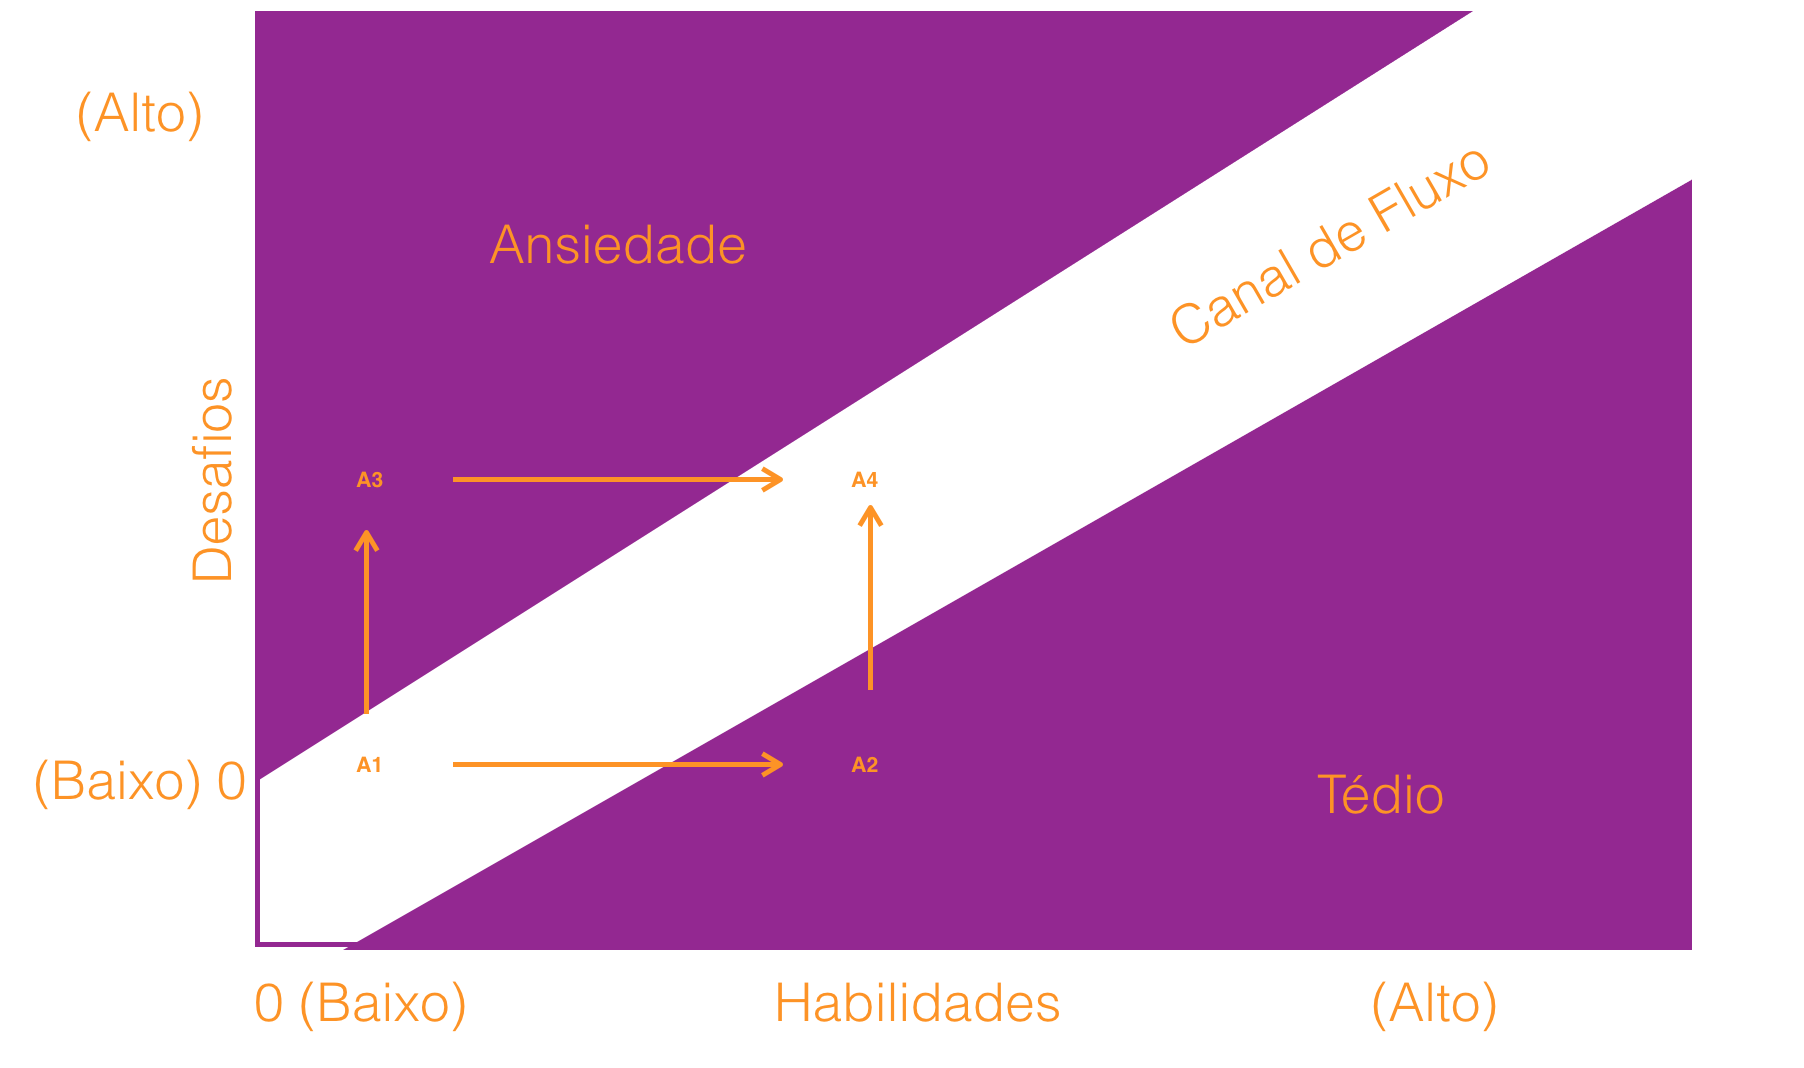
\includegraphics[keepaspectratio=true,scale=0.5]{figuras/flowfig.png}
	\caption{Diagrama do fluxo. Fonte: \cite{1990flow}.\label{flowfig}
}
\end{figure}


O diagrama representado na Fig. (\ref{flowfig}) exemplifica o pensamento de \cite{1990flow}. A letra A representa um indivíduo está iniciando uma atividade, a primeira vez que ele executa tal atividade, por exemplo, praticar um esporte novo ou um novo jogo de computador, ele tem pouca ou nenhuma habilidade, as primeiras ações da atividade geralmente não exigem grande esforço, o que é justo visto que A ainda não etm as habilidades necessárias para ações complicadas e difíceis. Neste ponto provalmente, como indica a figura ele está dentro do fluxo (A1), mas com a continuação da prática A melhora suas habilidades e praticar as mesmas ações que não exigem esforço torna a atividade entediante (A2). Caso encontre algum oponente mais prática A pode se sentir desafiado e um pouco decepcionado (A3) e se ele aceita o desafio e compete com um oponente e ganha ou alcança algum objetivo muito desejado ele volta ao estado de fluxo (A4). O autor define estado de fluxo como uma experiência ótima.

Entender a motivação humana é uma parte importante para criar estratégias efetivas de gamificação \cite{kumar2013gamification}, entender porque os jogadores continuam jogando e como trazer essa motivação para a gamificação é o primeiro passo de muitos que ainda serão dados se tratando de um assunto tão jovem como é a gamificação.

Gamification pode ser fácil de definir, enquanto não existe nenhum padrão de conceituação há uma concordância com a definição usualmente utilizada, no entanto uma visão mais profunda do tema exige maior desenvolvimento \cite{seaborn2015gamification}. 

Afim de obter uma visão diferente sobre gamificação  \cite{sailer2013psychological} investigou os diferentes elementos dos jogos  e como e porque eles podem acionar diferentes mecanismos motivacionais nos usuários, segundo os autores, do ponto de vista teórico  a gamificação tem o potencial de promover motivação em diferentes contextos. O autores encontraram três componentes principais quando se trata de motivação produzida por gamificação, o primeiro aspecto é a pessoa envolvida, é importante saber qual o público alvo. O segundo aspecto é o ambiente da gamificação, nesse aspecto as teorias motivacionais podem oferecer auxílio na construção destes ambientes. O terceiro aspecto é o contexto. O contexto pode ser visto como o conteúdo ou tópico de uma tarefa ou a situação geral em que se aplica a gamificação.

A motivação intrínseca é composta pelo desejo de novos desafios, testar a própria capacidade, adquirir novas habilidades e conhecimentos ou aproveitar uma tarefa. A motivação extrínseca está ligada ao desempenho afim de atingir um resultado, atingir um propósito a partir de um objetivo \cite{maican2016interactivia}, \cite{chou2015actionable}.


Como citado anteriormente, \cite{chou2015actionable} divide o octalysis em quatro partes. essa divisão figurativa que separa o framework em dois lados do cérebro (direito e esquerdo) está ligada as motivações intrínsecas e extrínsecas. Algumas falhas na aplicação de gamificação tem como responsáveis a enfase apenas nas motivações extrínsecas sem as motivações intrínsecas, excesso de pontos e medalhas e nenhuma criatividade, por exemplo \cite{maican2016interactivia}.

\subsection{Engajamento}

A gamificação almeja conciliar as duas motivações, com objetivo de aumentar a motivação e o engajamento \cite{muntean2011raising}, engajamento pode ser interpretado como o período de tempo em que temos muita ligação com algo, pode indicar desde a conexão entre um consumidor e um produto ou serviço até o tempo que um casal passa planejando passar o resto da vida juntos \cite{zichermann2011gamification}. O engajamento pode ser utilizado como medida de sucesso de uma gamificação. 


A figura (\ref{ciclofig}) representa o clico de engajamento, umas das unidades principais do modelo de gamificação proposto por \cite{kumar2013gamification}. O ciclo é de autoria de \cite{amy} combina loops de reforço e feedback positivo para manter o jogador engajado, utilizado em jogos progressão, por exemplo. A figura ilustra o pensamento expressado por \cite{amy} e \cite{kumar2013gamification}, deve-se iniciar motivando uma emoção no usuário, fazendo com que ele queira realizar a atividade diversas vezes, depois chamá-lo a realizar uma ação, motivá-lo com uma mistura de feedback e progresso e gatilhos integrados, com recompensar e trazer o jogador de volta e assim deixar ele sempre envolvido com o jogo. 

\begin{figure}[h]
	\centering
		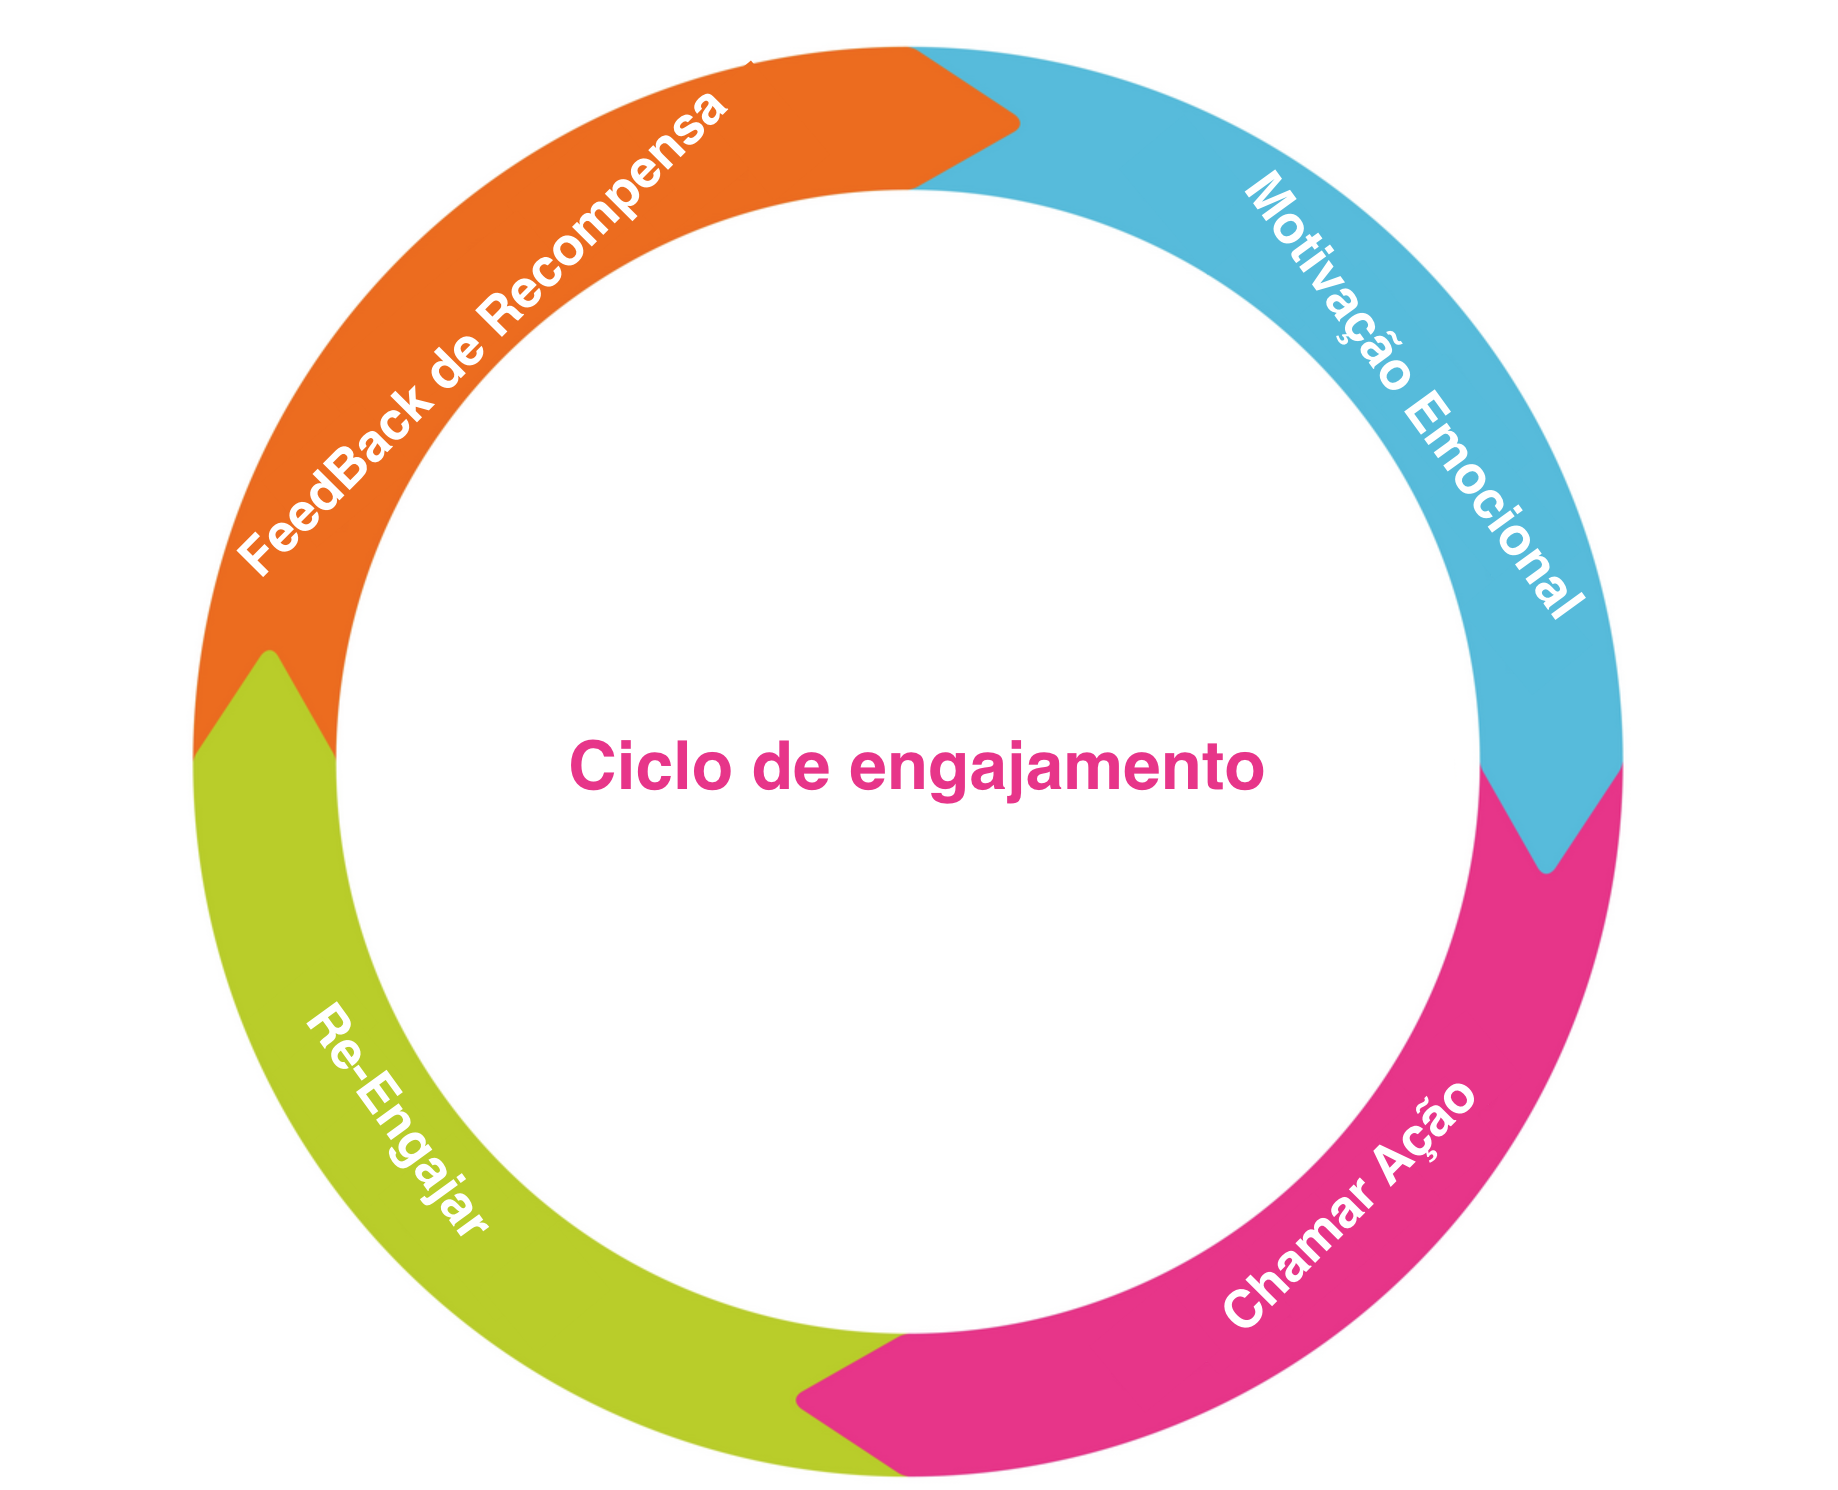
\includegraphics[keepaspectratio=true,scale=0.3]{figuras/ciclofig.png}
	\caption{Ciclo de Engajamento. Fonte: \cite{kumar2013gamification}.\label{ciclofig}
}
\end{figure}


Usando o contexto educacional \cite{fredericks2004school} apresenta três tipos de engajamento, comportamental, emocional e de aprendizagem.
O engajamento comportamental pode ser dividido de três maneiras, a primeira condutas positivas, como seguir as regras da sala de aula, a segunda definição dizer respeito sobre se envolver com aprendizado e as tarefas. A terceira diz respeito com participação em atividades escolares, como esportes. O engajamento emocional abrange as reações positivas e negativas dentro do contexto escolar. Atua criando laços entre a pessoa e a instituição e influencia na vontade de fazer o trabalho. O engajamento cognitivo  motiva a pessoa a exercer o esforço necessário, compreender idéias complexas e dominar as habilidades difíceis. A Figura


\section{Funifier}

O funifier é uma plataforma de gamificação, com presença global. Realiza gamificação na área de negócios, motivando equipes de vendas, aumentando o público de um site, age também na área educacional envolvendo os alunos virtualmente e permite também que seja criada uma gamificação do zero, a partir do contexto que o usuário necessite. A figura (\ref{globalfig}) demonstra a quantidade de escritórios da ferramenta pelo mundo.


\begin{figure}[h]
	\centering
		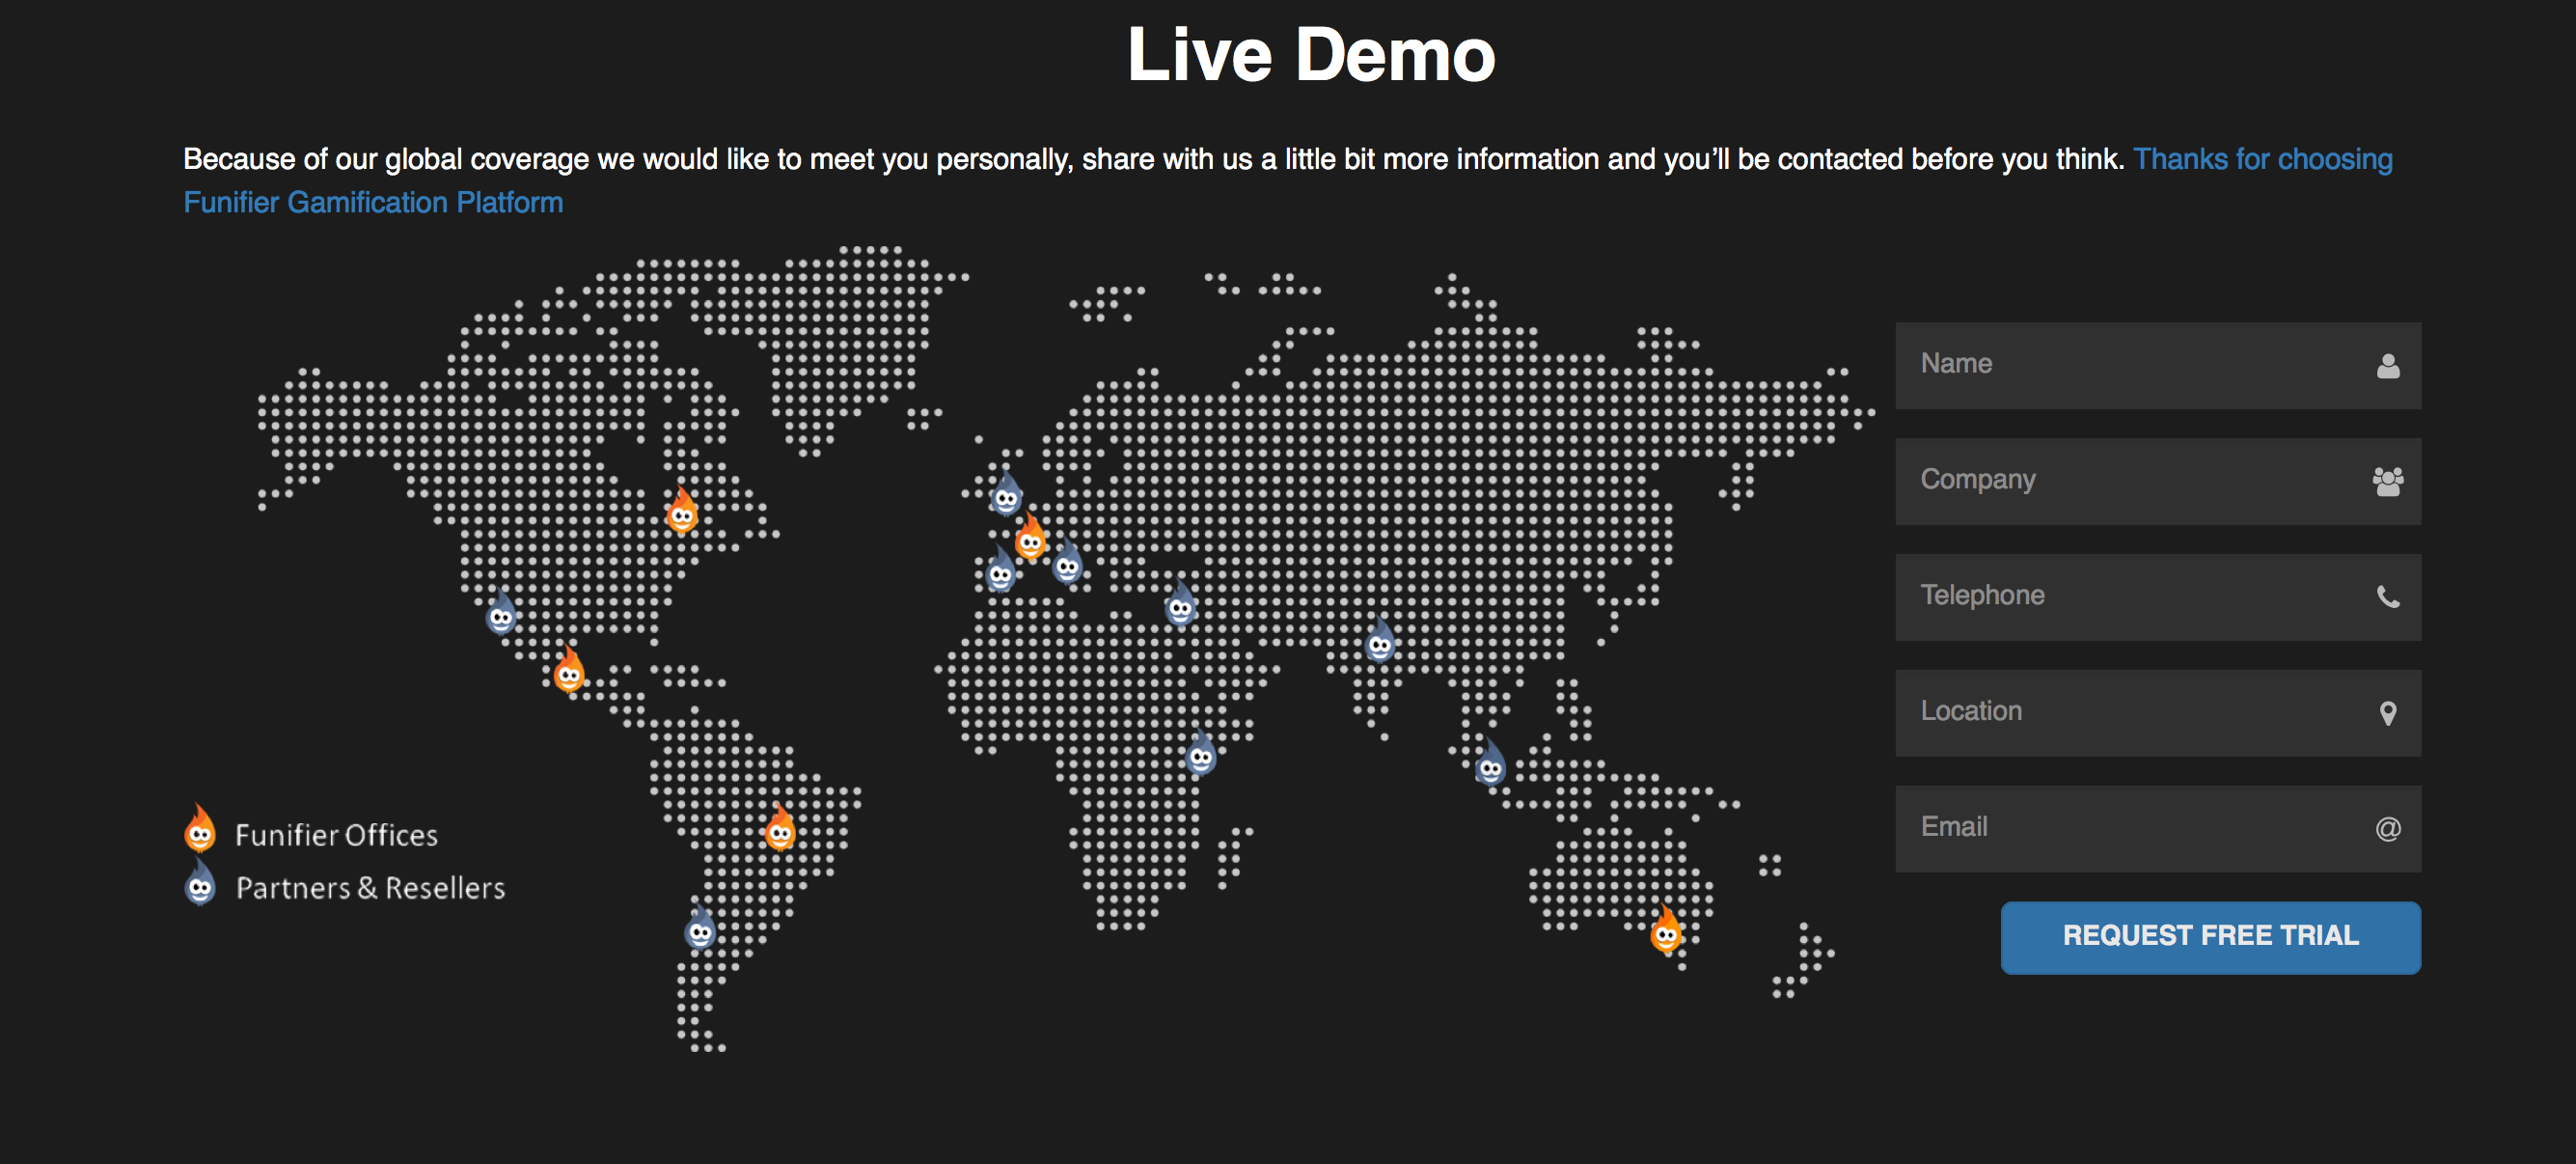
\includegraphics[keepaspectratio=true,scale=0.3]{figuras/globalfig.png}
	\caption{Escritórios da Funifier.\label{globalfig}
}
\end{figure}


Contém componentes pré fabricados que podem ser adicionados a sites e redes sociais, além da possibilidade de incluir desafios, notificações e outros aspectos relacionados a gamificação. A plataforma motiva o público alvo e os mantem engajados, de maneira que eles permaneçam visando conquistar seus objetivos. Mantém a privacidade do usuário, concedendo acesso de maneira seletiva, só acessa as gamificações quem tem o poder de fazê-lo. A figura (\ref{funifier}) foi retirada da página inicial da empresa e contém algumas informações a respeito da ferramenta.


\begin{figure}[h]
	\centering
		
\includegraphics[keepaspectratio=true,scale=0.3]{figuras/funifier.png}
	\caption{Componentes da Plataforma. Fonte: \cite{kumar2013gamification}.\label{funifier}
}
\end{figure}

\newpage

O funifier vai além de ofertar apenas os itens geralmente associados a gamificação, como pontos e troféus, a plataforma permite que você usufrua de mais de 90 diferentes técnicas de gamificação, possibilitando a adoção de estratégia mais adequado para o usuário. A figura (\ref{tecnicas}) representa a visão que usuário tem ao escolher as técnicas de gamificação que serão utilizadas no projeto que o usuário irá implantar.



\begin{figure}[h]
	\centering
		
\includegraphics[keepaspectratio=true,scale=0.3]{figuras/tecniques.png}
	\caption{Ciclo de Engajamento. Fonte: \cite{kumar2013gamification}.\label{tecnicas}
}
\end{figure}


